\begin{frame}[c]{In a Nutshell}

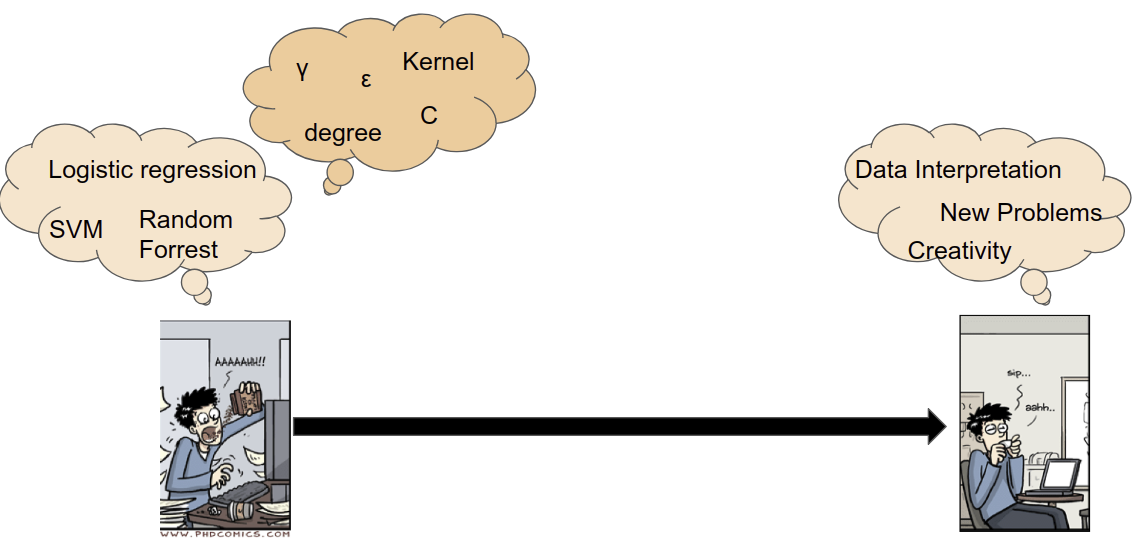
\includegraphics[width=0.99\textwidth]{images/automl_comic}

\end{frame}
%----------------------------------------------------------------------
%----------------------------------------------------------------------
\begin{frame}[c]{}

\huge
\centering
Why are you sitting here?

\bigskip


\includegraphics[scale=0.1]{images/hands.png}

\end{frame}
%----------------------------------------------------------------------
\begin{frame}[c]{}

\centering
\huge
Lecture 1:\\
Overview and Motivation
\end{frame}
%----------------------------------------------------------------------
%----------------------------------------------------------------------
\begin{frame}[c]{Overview}

What do we learn today?

\begin{itemize}
  \item Why ML does not scale up
  \item Design decisions in ML 
  \item What is AutoML? 
  \item Challenges in AutoML
  \item Risks of AutoML
  \item Meta-algorithmic hierarchy 
  \item Organization of the course
\end{itemize}

\end{frame}
%-----------------------------------------------------------------------
%----------------------------------------------------------------------
\begin{frame}[c]{Machine Learning}

\centering
\textit{``Machine learning is the science of getting computers to act\\
 without being explicitly programmed.''}

\hfill by Andrew Ng

\end{frame}
%-----------------------------------------------------------------------
%----------------------------------------------------------------------
\begin{frame}[c]{Machine Learning}

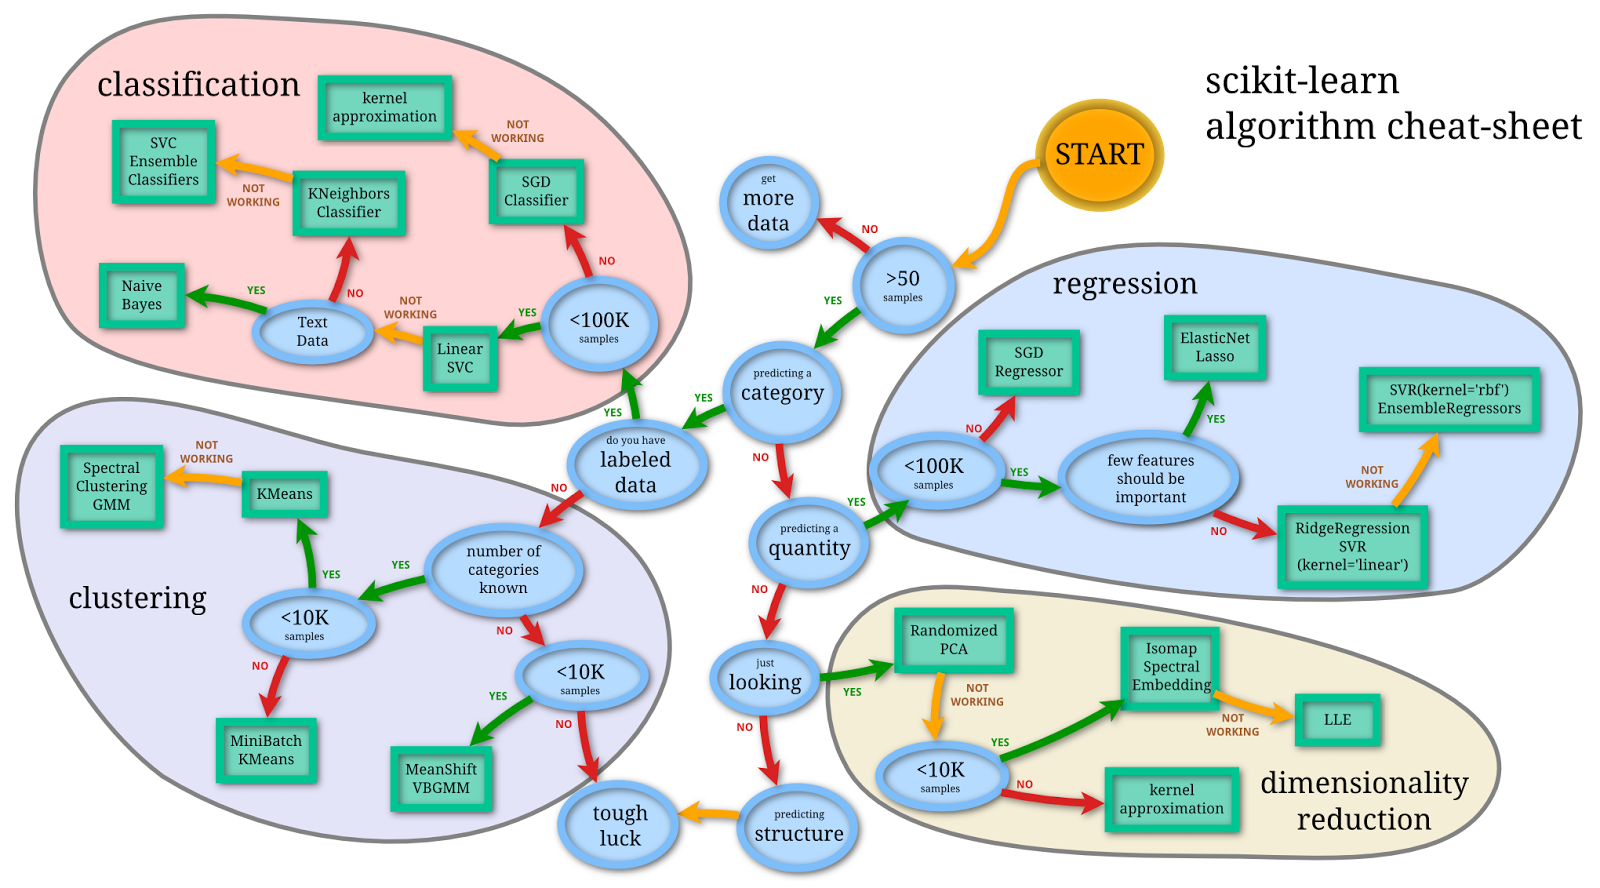
\includegraphics[width=1.0\textwidth]{images/sklearn-cheat}

\end{frame}
%-----------------------------------------------------------------------
%----------------------------------------------------------------------
\begin{frame}[c]{Machine Learning Workflow}

\centering
\tikzstyle{activity}=[rectangle, draw=black, rounded corners, text centered, text width=8em, fill=white, drop shadow]
\tikzstyle{wideactivity}=[rectangle, draw=black, rounded corners, text centered, text width=10em, fill=white, drop shadow]
\tikzstyle{data}=[rectangle, draw=black, text centered, fill=black!10, text width=8em, drop shadow]
\tikzstyle{myarrow}=[->, thick]
\begin{tikzpicture}[node distance=5cm,thick]
	\node (Train) [data] {DataSet $D_{\text{train}}$};
	\node (Fit) [activity, below of=Train, node distance=2cm] {Train model based on $D_{\text{train}}$};
	\draw[myarrow] (Train) -- (Fit);
	
	\pause
	
	\node (Test) [data, right of=Train] {DataSet $D_{\text{val}}$};
	\node (Eva) [activity, below of=Test, node distance=2cm] {Evaluate model on $D_{\text{val}}$};
	\draw[myarrow] (Fit) -- (Eva);
	\draw[myarrow] (Test) -- (Eva);
	
	\pause
	
	\node (user) [data, below of=Eva, node distance=2cm] {User};
	\draw[myarrow] (Eva) to node[right] {Performance} (user);
	
	\pause
	
	\node (Hyper) [activity, left of=user] {Adapt\\ Hyperparameters};
	\draw[myarrow] (user) to (Hyper);
	\draw[myarrow] (Hyper) to (Fit);
	
\end{tikzpicture}


\pause
 
\bigskip
\bigskip
$\leadsto$ Users indirectly teach machines how to learn.

\end{frame}
%-----------------------------------------------------------------------
%----------------------------------------------------------------------
\begin{frame}[c]{Machine Learning does not scale up}

\begin{itemize}
  \item Basics in machine learning are not hard to grasp
  \smallskip
  \item Achieving state-of-the-art performance is quite hard
  \smallskip
  \item Design decisions are (sometimes) unintuitive and\\ require a lot of expertise
  \begin{itemize}
    \item making these design decisions is a tedious and error-prone task
  \end{itemize}
  \smallskip
  \item Many experts are employed in ML these days
  \smallskip
  \item Nevertheless, developing a new ML-applications takes time
  \smallskip
  \item The job market for ML experts is nearly empty
\end{itemize}

\bigskip

\textit{``I'd like to use machine learning, but I can't invest much time''}

\hfill Zoubin Gharamani


\end{frame}
%-----------------------------------------------------------------------
%----------------------------------------------------------------------
\begin{frame}[c]{Design Decisions in Machine Learning}

What could be design decisions for applying ML to a new dataset?
\hands

\pause

\begin{itemize}
  \item Choice of machine learning algorithm
  \begin{itemize}
    \item SVM, random forest, deep neural network?
  \end{itemize}
  \pause
  \item Hyperparameters of machine learning algorithms
  \begin{itemize}
    \item SVM: C, gamma, kernel, \ldots?
  \end{itemize}
  \pause
  \item Architecture of a neural network
  \begin{itemize}
    \item $\#$layers, $\#$neurons, activation function, \ldots 
  \end{itemize}
  \pause
  \item Data preprocessing
  \begin{itemize}
  	\item data cleanup, missing data imputation, feature selection, \ldots  
  \end{itemize}
  \pause
  \item anomaly detection
  \item allocation of computational resources
  \item \ldots
\end{itemize}

\medskip
$\leadsto$ All these design decisions have to be made for each new dataset.

\end{frame}
%-----------------------------------------------------------------------
%----------------------------------------------------------------------
\begin{frame}[c]{A simple Example with $k$-NN}

\centering
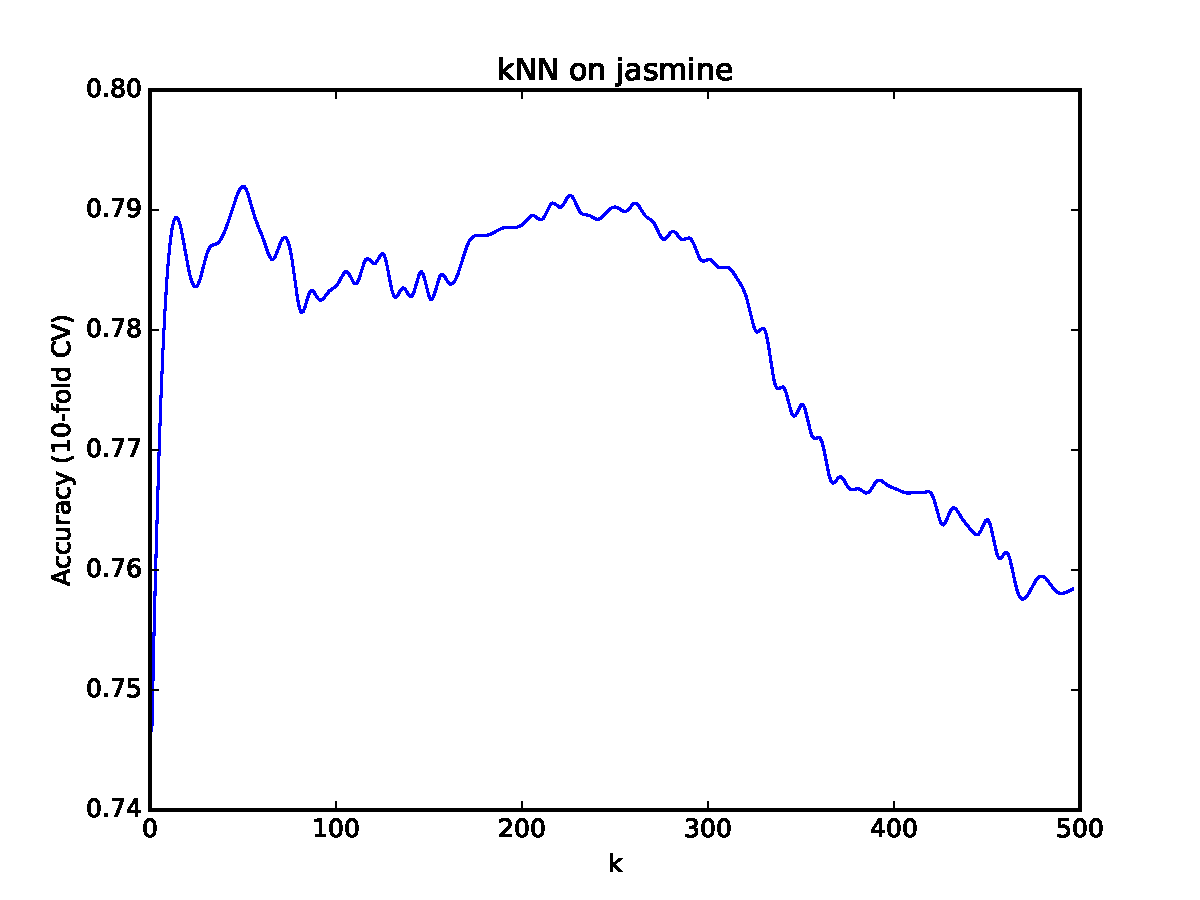
\includegraphics[width=0.6\textwidth]{images/kNN-jasmine}

\begin{itemize}
  \item $k$-nearest neighbors is one of the most trivial ML algorithms
  \item Size of neighbourhood ($k$) is very important for its performance
  \item The performance function depending on $k$ is quite complex\\ (not at all convex)
\end{itemize}

\end{frame}
%-----------------------------------------------------------------------
%----------------------------------------------------------------------
\begin{frame}[c]{Goal of AutoML}

\begin{block}{AutoML}
The goal of AutoML is to automate all parts of machine learning (as needed)
to \emph{support} users efficiently building their machine learning applications.
\end{block}

\bigskip

\begin{block}{AutoML System}
Given
\begin{itemize}
  \item a dataset
  \item a task (e.g., regression or classification)
  \item a performance metric (e.g., accuracy or RMSE)
\end{itemize}
an AutoML system automatically determines the approach 
that performs best for this particular application.
\end{block}

\end{frame}
%-----------------------------------------------------------------------
%----------------------------------------------------------------------
\begin{frame}[c]{AutoML in Research}

AutoML enables:

\begin{enumerate}
  \item more efficient research
  \begin{itemize}
    \item AutoML has shown on subproblems to outperform human experts
  \end{itemize}
  \pause
  \smallskip
  \item more systematic research
  \begin{itemize}
    \item humans tend to be unsystematic which leads to errors
  \end{itemize}
  \smallskip
  \pause
  \item more reproducible research
  \begin{itemize}
    \item since AutoML is systematic and human's unsystematic approaches cannot be reproduced 
  \end{itemize}
  \item broader use of ML also in other disciplines
  \begin{itemize}
    \item ML should not be limited to computer scientists;
    \item the most amazing applications of ML is often done\\ by either interdisciplinary teams or even non-computer scientists
  \end{itemize}
\end{enumerate}

\end{frame}
%-----------------------------------------------------------------------
%----------------------------------------------------------------------
\begin{frame}[c]{Challenges in AutoML}

\begin{enumerate}
  \item Design decisions have to be made for each dataset again
  \item Training of a single ML model can be quite expensive\\
  		(e.g., hours, days or weeks)
  \begin{itemize}
    \item[$\leadsto$] often, we cannot try a many design decisions
  \end{itemize}
  \item the mathmatical relation between design decisions\\ and performance is (often) unknown
  \begin{itemize}
    \item[$\leadsto$] gradient-based optimization is not directly possible
  \end{itemize}
  \item optimization in highly complex spaces
  \begin{itemize}
    \item incl. categorical choices, continuous parameters,\\ conditional dependencies
  \end{itemize}
  
\end{enumerate}

\end{frame}
%-----------------------------------------------------------------------
%----------------------------------------------------------------------
\begin{frame}[c]{Risks of AutoML}

What could be risks of AutoML?
\hands
\pause

\begin{enumerate}
  \item Users apply AutoML without understanding anything.
  \begin{itemize}
    \item Users might wonder why (Auto-)ML does not perform well\\ after they passed poor data. 
  \end{itemize}
  \pause
  \item The users over-trust the AutoML too much.
  \begin{itemize}
    \item humans might not use human reasoning skills and do not second guess machine decisions
  \end{itemize}
  \pause
  \item We enable non-ML experts to use ML\\ without knowing the risks and consequences of ML.
  \pause
  \item Could result in deployment of \ldots
  \begin{itemize}
    \item inaccurate ML models due to lack of understanding of statistical concepts, e.g., sampling bias, overfitting, concept drift, \ldots
    \item biased and unfair models due to lack of understanding ethical practices and use of features such as gender and race for predicting outcomes
  \end{itemize}
\end{enumerate}

See \textit{\href{https://arxiv.org/abs/1902.06804}{Democratisation of Usable Machine Learning in Computer Vision}}

\end{frame}
%-----------------------------------------------------------------------
%----------------------------------------------------------------------
\begin{frame}[c]{Snipped of Meta-Algorithmic Hierarchy}


Meta-algorithmic approaches

\begin{itemize}
  \item[$\subset$] AutoAI
  \pause
  \begin{itemize}
		\item[$\subset$] AutoML
		\pause
		\begin{itemize}
		 	\item[$\subset$] Hyperparameter optimization (HPO)
		 	\pause
		 	\item[$\subset$] Neural architecture search (NAS)\\
		 	   \hspace{1em} Google sometimes claims: AutoML $==$ NAS\\
		 	   \hspace{1em} but that's wrong!
		 	\pause
		 	\item[$\subset$] Meta-learning\\
		\end{itemize}
		\pause
		\item[$\subset$] Algorithm configuration
	\end{itemize}
	\pause
	\item[$\subset$] Search-based software engineering
\end{itemize}

\end{frame}
%-----------------------------------------------------------------------
%----------------------------------------------------------------------
\begin{frame}[c]{Goals of the Lecture}

You will be able to \ldots
\begin{enumerate}
  \item use AutoML tools
  \smallskip
  \item develop AutoML tools
  \smallskip
  \item have a good overview over the state-of-the-art in AutoML
  \smallskip
  \item do research on AutoML yourself
  \begin{itemize}
    \item perfect opportunity to do a master project or thesis with us afterwards
  \end{itemize}
\end{enumerate}

\end{frame}
%-----------------------------------------------------------------------
%----------------------------------------------------------------------
\begin{frame}[c]{Course Overview}

\begin{itemize}
	\item Introduction
	\item Background
	\begin{itemize}
		\item Design spaces in ML
		\item Experimentation and visualization
	\end{itemize}
	\item Hyperparameter optimization (HPO)
	\begin{itemize}
	  \item Bayesian optimization
	  \item Other black-box techniques
	\end{itemize}
	\item Speeding up HPO with multi-fidelity optimization
	\item Pentecost (Holiday) -- no lecture
	\item Architecture search I + II
	\item Meta-Learning
	\item Learning to learn $\&$ optimize
	\item Beyond AutoML: algorithm configuration and control
	\item Project announcement and closing
\end{itemize}


\end{frame}
%----------------------------------------------------------------------
%----------------------------------------------------------------------
\begin{frame}[c]{Team - Lectures}

\begin{columns}[T]
\column{0.5\textwidth}

\centering
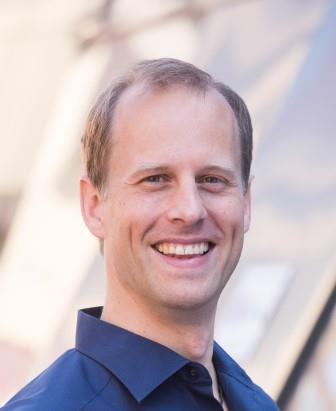
\includegraphics[width=9em]{images/team/frank_small}

Prof. Dr. Frank Hutter

\column{0.5\textwidth}
\centering
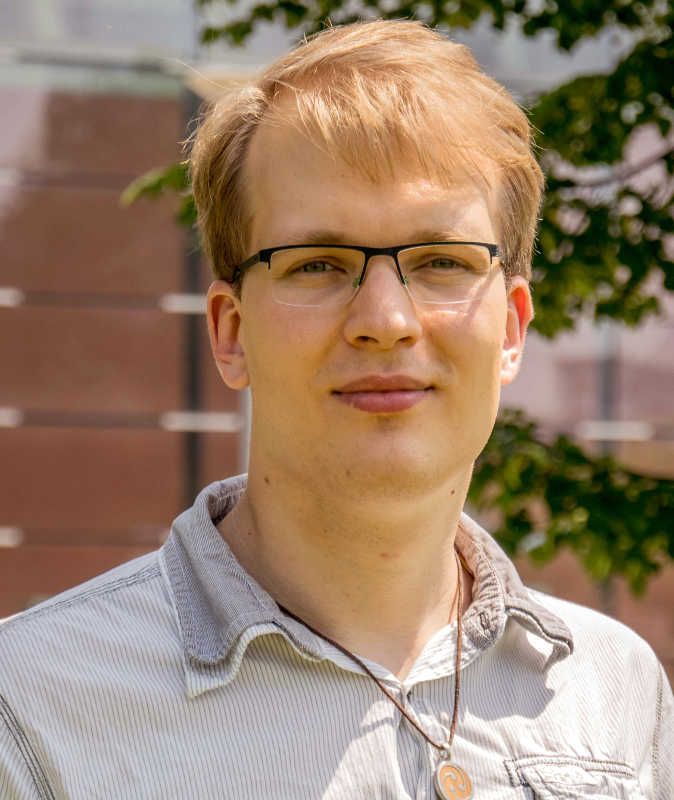
\includegraphics[width=9em]{images/team/marius}

Dr. Marius Lindauer

\end{columns}

\end{frame}
%----------------------------------------------------------------------
%----------------------------------------------------------------------
\begin{frame}[c]{Team -- Exercise}

\begin{columns}[T]

\column{0.3\textwidth}
\centering
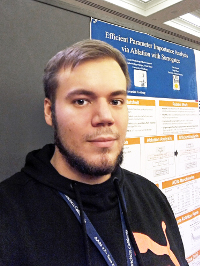
\includegraphics[height=9em]{images/team/biedenkapp}
André Biedenkapp
\column{0.3\textwidth}
\centering
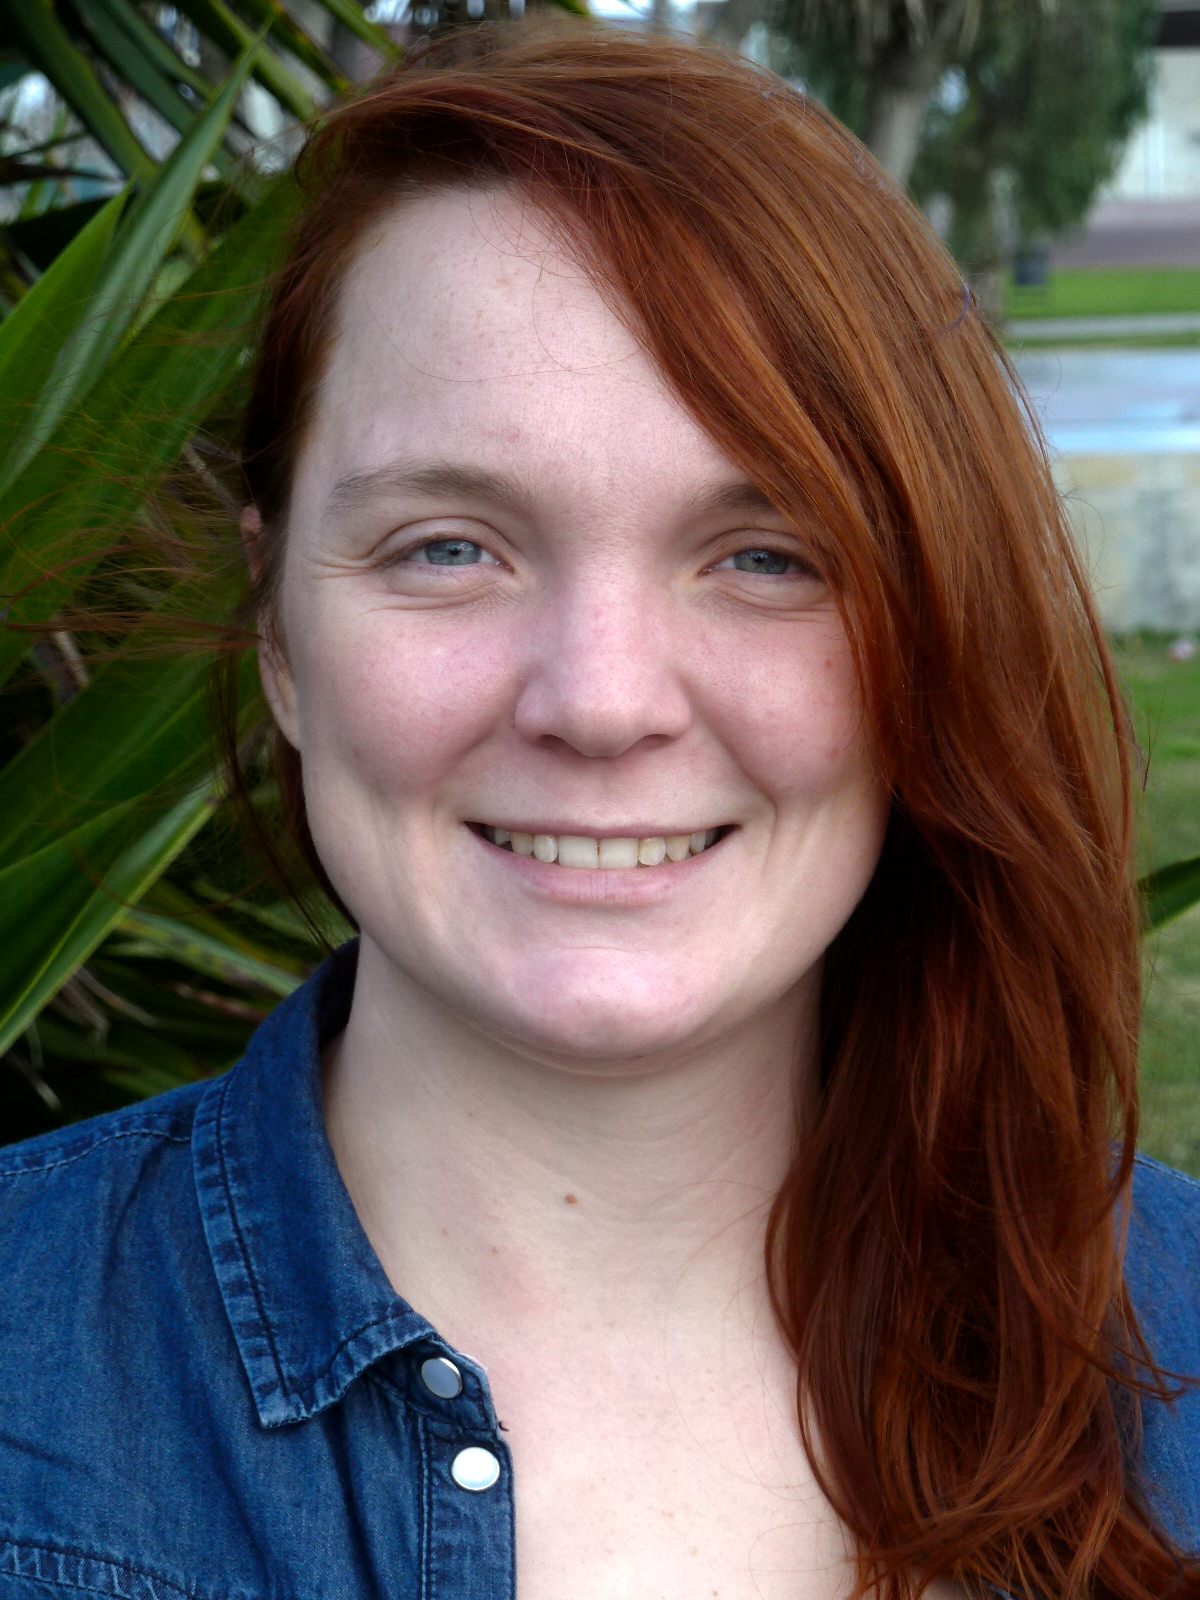
\includegraphics[height=9em]{images/team/eggensperger_small}
Katharina Eggensperger
\column{0.3\textwidth}
\centering
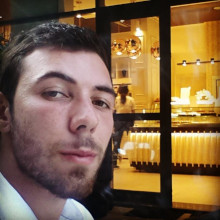
\includegraphics[height=9em]{images/team/arber_small}
Arber Zela

\end{columns}

\end{frame}
%----------------------------------------------------------------------
%----------------------------------------------------------------------
\begin{frame}[c]{Organization (Lectures)}

\begin{itemize}
  \item $6$ ECTS
  \item Every week at Monday: 14:15 (s.t) - 15:45\\ (Building: 106 Room: SR 00 007)
  \item \emph{Interactive} Lecture 
  \begin{itemize}
    \item We will ask you questions in the lectures
    \item Kahoot quiz at the end of each lecture
  \end{itemize}
  \item Course material on our homepage\\
  		{\small \url{ml.informatik.uni-freiburg.de/teaching/ss2019/automl/}}
  \item Slides will be online before the lectures
  \item No video recording!
\end{itemize}

\end{frame}
%-----------------------------------------------------------------------
%----------------------------------------------------------------------
\begin{frame}[c]{Organization (Exercises)}

\begin{itemize}
  \item Every Friday at: 14:15 - 15:45\\ (Building: 106 Room: SR 00 007)
  \begin{itemize}
    \item No meeting this week, but first exercise sheet!
  \end{itemize}
  \item Every week new exercise sheet and discussion of last exercise
  \item Most exercises will be practical, i.e., you have to implement something
  \item Team work allowed, max team size: 2! 
  \item Cheating:
  \begin{itemize}
    \item First time cheating: $0$ points for exercise
    \item Second time cheating: failing the course
  \end{itemize}
  \item You have to obtain at least $50\%$ points in the exercises  
  \item The number of points per sheet will slightly increase over time
  \item Submit via bitbucket (git)
\end{itemize}

\end{frame}
%-----------------------------------------------------------------------
%----------------------------------------------------------------------
% \begin{frame}[c]{Exceptions (tentative)}
% 
% \begin{itemize}
% 	\item No lectures and exercises during vacations and holidays\\ (1. Nov, 25. Dec, 27. Dec, 01. Jan, 03. Jan)
% 	\item Switching lecture and exercise slot 11. Dec and 13. Dec
% 	\item Last lecture at 05. Feb
% \end{itemize}
% 
% \end{frame}
%-----------------------------------------------------------------------
%----------------------------------------------------------------------
\begin{frame}[c]{Requirements}

\begin{itemize}
  \item Knowledge in \alert{Machine Learning} (strongly recommended)
  \begin{itemize}
    \item Classification, regression, clustering, decision tree, training-test split, cross validation, pre-processing \ldots
  \end{itemize}
  \pause
  \item Knowledge in \alert{Deep Learning} (strongly recommended)
  \begin{itemize}
    \item feed-forward network, recurrent network, convolutions, learning rates, regularization, \ldots 
  \end{itemize}
  \pause
  \item Experience in \alert{Python and git} (recommended)
  \begin{itemize}
    \item nearly all exercises will require 
    that you implement something in~Python and submit the solution to a git repo
  \end{itemize}
\end{itemize}

\end{frame}
%-----------------------------------------------------------------------
%----------------------------------------------------------------------
\begin{frame}[c]{Final Oral Exam}

\begin{itemize}
  \item Implement a larger project (worth $1-2$ weeks fulltime)
	\begin{itemize}
		\item No teamwork!
	\end{itemize}
  \item Exam
	\begin{itemize}
		\item Present the project in the first $15$ minutes\\ (including some questions from us)
		\item Answer questions about further course material in the second $15$ minutes
	\end{itemize}	
  \item tentative date: end of September
\end{itemize}

\end{frame}
%----------------------------------------------------------------------
%----------------------------------------------------------------------
\begin{frame}[c]{Resources}

\begin{itemize}
  \item To get a deep understanding of AutoML, you should also read some literature 
  \item We will provide links to papers at the end of each lecture
  \item New AutoML book: \url{https://www.automl.org/book/}
  \begin{itemize}
    \item Draft online available
  \end{itemize}
\end{itemize}

\end{frame}
%----------------------------------------------------------------------
%----------------------------------------------------------------------
\begin{frame}[c]{Chances and Risks}

AutoML is an advanced lecture and we modify it each time.

\bigskip
\pause

Chances:
\begin{itemize}
  \item All presented topics are close to state-of-the-art;\\there is active research on these topics  
  \item The course will provide a solid background\\ for doing a master project/thesis in our group 
\end{itemize}

\medskip

Risks:
\begin{itemize}
  \item You will find some typos and issues in the slides;\\ please tell us if you find something
  %\item Workload could be very high for you -- we have no experience with the exercises yet
\end{itemize}

\medskip
\pause
$\to$ Give us some feedback and we will improve the course!

\medskip
\pause
Note: AutoML was already partially covered in our old lecture ML4AAD. 
If you successfully attended ML4AAD, please don't attend AutoML.

\end{frame}
%-----------------------------------------------------------------------
%----------------------------------------------------------------------
\begin{frame}[c]{Introduce yourself!}

\begin{itemize}
  \item Why have you chosen this course?
  \medskip
  \item Background knowledge? (ML, DL, \ldots)
  \medskip 
  \item Experience with such problems?
\end{itemize}

\bigskip
\centering

\includegraphics[scale=0.1]{images/hands.png}

\end{frame}
%-----------------------------------------------------------------------
%----------------------------------------------------------------------
% \begin{frame}[c]{Exercise I }
% 
% \begin{block}{Task}
% \begin{enumerate}
% 	\item Identify $2$ (known) algorithms which have tunable parameters and briefly describe these parameters
% 	\item Describe a manual way to tune the parameters and approximate the effort you would need to do this on an example
% 	\item Analyze the runtime complexity of the algorithms
% \end{enumerate}
% \end{block}
% 
% \alert{Submission due 02.11. (23:59 GMT)}\\
% Submit at ILIAS : \url{https://ilias.uni-freiburg.de/goto.php?target=crs_465155&client_id=unifreiburg}
% %Send to: \url{lindauer@cs.uni-freiburg.de}\\
% %with subject: \texttt{[MLOAD Excercise I] $<$your name$>$} 
% 
% \end{frame}
%-----------------------------------------------------------------------
% %----------------------------------------------------------------------
% \begin{frame}[c]{}
% 
% 
% 
% \end{frame}
% %-----------------------------------------------------------------------

